%% LyX 2.0.4 created this file.  For more info, see http://www.lyx.org/.
%% Do not edit unless you really know what you are doing.
\documentclass[oneside,dutch]{amsart}
\usepackage[T1]{fontenc}
\usepackage[latin9]{inputenc}
\usepackage[a4paper]{geometry}
\geometry{verbose,tmargin=3cm,bmargin=3cm,lmargin=2cm,rmargin=2cm}
\setlength{\parskip}{\smallskipamount}
\setlength{\parindent}{0pt}
\usepackage{amsthm}
\usepackage{graphicx}
\graphicspath{{Figures/}}

\makeatletter
%%%%%%%%%%%%%%%%%%%%%%%%%%%%%% Textclass specific LaTeX commands.
\numberwithin{equation}{section}
\numberwithin{figure}{section}

\makeatother

\usepackage{babel}
\begin{document}

\title{Profielwerkstuk}


\author{N.G. Schultheiss}

\maketitle

\section{Inleiding}

\noindent \begin{center}
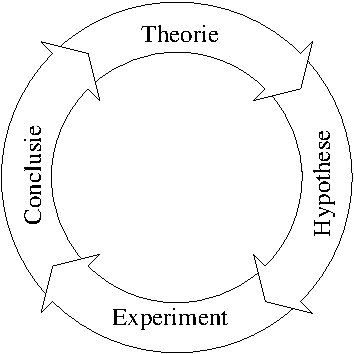
\includegraphics[scale=0.75]{cirkel}
\par\end{center}

Een HiSPARC-profielwerkstuk is te beschouwen als een wetenschappelijk
onderzoek. Hierboven is een eenvoudig model voor een wetenschappelijk
onderzoek te vinden. Omdat dit model in een cirkel is te beschrijven,
is het van belang om van te voren na te denken over het begin en het
eind van je onderzoek.

Een goede start is het formuleren van een onderzoeksvraag, die in
je onderzoek beantwoord wordt (bijvoorbeeld: Wat is de vorm van de
Aarde?). Het is ook mogelijk om deze onderzoeksvraag als stelling
op te schrijven (bijvoorbeeld: De Aarde is rond.). In de praktijk
is het eenvoudiger om een stelling of hypothese te bevestigen of te
weerleggen dan om een vraag te beantwoorden.

Meestal zal een hypothese pas geformuleerd kunnen worden, nadat je
bestudeerd hebt wat er al onderzocht is. Onderzoek in het verleden
is op allerei wijzen in theorie�n vastgelegd. Meestal leidt het bestuderen
van een theorie tot een nieuwe onderzoeksvraag / hypothese.

Als bekend is welke hypothese je wilt onderzoeken, moet er een goede
experimentele opzet worden gekozen. Als het experiment uitgevoerd
is, zijn er experimentele gegevens beschikbaar. Hier valt een conclusie
uit te trekken. In een discussie kunnen de gevolgen voor een theorie
worden besproken.

Het bijhouden van een logboek, waarin je al je gedachten en waarnemingen
zet, geeft een goede start voor het verslag. In het verslag doe je,
zoals het woord al zegt, verslag van je onderzoek. In het verslag
moeten de volgende punten behandeld worden:
\begin{enumerate}
\item Inleiding, leg hierin uit hoe je tot je onderzoek gekomen bent en
wat je hypothese is.
\item De opzet van je experiment. Leg hierin uit hoe je je hypothese wilt
toetsen.
\item Resultaten. Persoonlijk wil ik de resultaten van het experiment scheiden
van de uitwerking. Deze waarnemingen worden hier beschreven.
\item Uitwerking. De uitwerking van de resultaten hangt ten dele af van
de kennis van de experimentator. Deze is dus minder objectief dan
de waarnemingen.
\item Conclusie. Uit de uitwerking is een conclusie te trekken.
\item In de discussie kan de conclusie worden verwerkt in een nieuwe theorie.
Eventueel kan hier ook worden aangegeven of de conclusie altijd uit
de metingen te trekken valt.
\end{enumerate}

\section{Een detector profielwerkstuk}

In een detector profielwerkstuk bestuderen we eigenschappen van de
detector. Er is bijvoorbeeld te onderzoeken of de meetwaarden van
de temperatuurafhangen.
\end{document}
